\documentclass{article}

\usepackage{graphicx}
\usepackage{wrapfig}
\usepackage{subcaption}
\usepackage[margin=1in]{geometry}
\usepackage{amsmath} % or simply amstext
\usepackage{amssymb}
\usepackage{siunitx}
\usepackage{booktabs}
\usepackage[export]{adjustbox}
\newcommand{\angstrom}{\textup{\AA}}
\newcommand{\colormap}{jet}  % colorbar to use
\usepackage{cleveref}
\usepackage{booktabs}
\usepackage{gensymb}
\usepackage{float}
\usepackage{xr}
\usepackage{setspace}
\doublespacing

\externaldocument[S-]{Supporting_Information}

\title{Statistical Inference of Transport Mechanisms and Long Time Scale Behavior from Time Series 
       of Solute Trajectories in Nanostructured Membranes.}

\author{Benjamin J. Coscia, Christopher P. Calderon, Michael R. Shirts} 

\begin{document}

  \graphicspath{{./figures/}}
  \maketitle
  
  % BJC2: I'm not putting a lot of effort into the introduction since I'll only write
  % an abbreviated form for my dissertation. I'll work on the intro after my defense.  
  %MRS7: sounds good, I won't look at this today.

  \section{Introduction}
  
%  There is a need for highly selective membranes in order to perform efficient 
%  separations of components of complex aqueous streams.
%  %MRS2: add some more examples (When you get around to it).
%  \begin{itemize}
%    \item Organic micropollutants
%    \item Desalination and boric acid removal from seawater.
%    \item While many researchers focus on membrane permeability, we may be 
%    able to reduce costs of commercial nanofiltration and reverse osmosis with
%    higher selectivity.~\cite{werber_materials_2016}
%  \end{itemize}
%
%%  \noindent Amphiphilic molecules are capable of self-assembling into ordered nanostructures.
%%  \begin{itemize}
%%    \item 
%%  \end{itemize}
%
%  Lyotropic liquid crystals (LLC) are a class of amphiphilic molecules whose ordered phases
%  can be cross-linked into mechanically strong membranes capable of highly selective
%  separations.
%  \begin{itemize}
%    \item The shape of the LLC monomers and water content dictates the ordered phase 
%    that they form. There are two phases of particular interest for membrane applications.
%  	\item H\textsubscript{II} phase lyotropic liquid crystals are characterized by 
%  	hexagonally packed, straight, pores while the Q\textsubscript{I} phase consists of
%  	a tortuous network of 3D interconnected pores. 
%  	\item In both cases the pores are uniform in size with radii on the order of 1 nm
%    %MRS2: is it really a molecular weight cutoff?
%    %BJC2: is molecular size better? Obviously there are other factors like shape, but I don't want to get into that
%  	giving them a very strict molecular size cut-off.
%	\item Additionally, they have the potential to disrupt conventional membrane separation
%	techniques by being selective based not only on size and charge, but on chemical
%	functionality as well.
%	\item Their pores are lined with LLC monomer functional groups which can potentially
%	be designed to interact with solutes in a chemically-specific manner
%  \end{itemize}
%
%  There are limits to what we can learn from experiment about LLC membrane design.
%  \begin{itemize}
%    \item Experimental observables like permeability and selectivity allow us to speculate
%    about the molecular origins of separation processes.
%    %MRS2: not quite sure what you mean below?
%    \item This drives an empirical design approach which can potentially neglect key
%    interactions which influence selectivity.
%    \item LLC membranes have been shown to exhibit selectivities which cannot be fully 
%    explained by relatively simple macroscopic models. 
%  \end{itemize}
%  
%  Molecular Dynamics (MD) simulations can give us mechanistic insights with atomistic 
%  resolution so that we can intelligently design new membranes for solute-specific 
%  separations.
%  \begin{itemize}
%    \item In our previous work, we built a detailed atomistic model which we used
%    to understand the nanoscopic structure of an LLC Membrane.~\cite{coscia_understanding_2019}
%    \item We also used the model in order to gain a qualitative understanding of 
%    trapping mechanisms which lead to subdiffusive transport behavior.~\cite{coscia_chemically_2019}
%  \end{itemize}
%
%  Unfortunately, the timescales that we can simulate with MD are insufficient to be
%  able to make well-converged predictions of macroscopic transport properties 
%  traditionally used to characterize membranes in the lab.
%  \begin{itemize}
%    %MRS2: would be good to get this next point into the first line of a paragraph, since it's quite important. 
%    \item However, if we use descriptive stochastic models that can capture solute
%    dynamics, then we could project long timescale behavior in addition to gaining
%    a deeper understanding of solute behavior on short timescales.
%  \end{itemize}
  
  %%%%%%%%%%%%%%%%%%%%%%%% Thesis chapter starts here %%%%%%%%%%%%%%%%%%%%%%%%%%%%%%%%
  
  In our previous 
%MRS:work
study,
  we designed two different approaches which used
  solute time series in order to parameterize stochastic models that could be used
  to project transport on much longer timescales. In our first approach we modeled 
  solute trajectories as subordinated fractional Brownian and L\'evy motion, called
  the anomalous diffusion (AD) model. We generated solute trajectories by generating
  a series of anti-correlated hops separated by random periods of entrapment drawn 
  from a power law distribution. Our second approach treated solute motion as a Markov
  state model with state-dependent dynamics, called the Markov state-dependent dynamical
  model (MSDDM). We parameterized the state transition probabilities between
  each of eight discrete states as well as the solute dynamics within each of these
  states. We generated stochastic trajectory realizations by drawing a state
  sequence based on the transition probability matrix and incorporating the state dynamics
  while solutes were trapped in each state.
  
  Although both models had reasonable success at predicting solute mean squared 
  displacements (MSDs) on MD simulation timescales, they had shortcomings.
  The MSDDM failed to reproduce the hopping and trapping behavior that
  characterizes solute center-of-mass trajectories in our MD simulations.
  The AD model did not suffer this qualitative shortcoming, but the persistent 
  curvature of the predicted MSD curves suggested that the model might 
  underestimate MSDs on long timescales. The formulation of both models required
  careful examination and characterization of the interactions and dynamics exhibit
  by MD trajectories which required considerable human effort.
  
  In this work we attempt to minimize human effort by applying the infinite hidden 
  Markov Model (IHMM), a nonparameteric Bayesian classification technique, in order to 
  automatically detect and infer the parameters of an unknown number of latent
  autoregressive (AR) modes present in solute center-of-mass time series trajectories.
  We aim to address two primary scientific questions with this work. First, we want
  to know if the IHMM algorithm can help researchers efficiently uncover underlying
  transport mechanisms which give rise to different solute dynamical behavior.
  Second, we want to evaluate the ability of our model to reproduce solute trajectories
  in a stochastic manner so that we can use it to predict macroscopic transport 
  properties which would otherwise require much longer MD simulations.
  
  We use the parameters of the states identified by the IHMM in order to infer 
  dominant solute-membrane interactions and transport mechanisms. We cluster similar 
  state parameters in order to reduce the state space and to understand which segments 
  of the solute trajectories exhibit similar behavior. We support our mechanistic 
  hypotheses via quantitative comparison to various physical membrane properties and
  solute-membrane interactions.
  
  Because independent solute trajectories generated by MD simulations share 
  similar state dynamics, we can use the IHMM to generate stochastic trajectory 
  realizations which sample from all behavior exhibited by MD. We verify that our
  stochastic realizations reproduce the expected hopping and trapping behavior 
  exhibited by MD. We quantitatively validate these trajectories by comparing 
  their mean squared displacement (MSD) to MSDs measured by MD.
    
  \section{Methods}
    
  We ran all MD simulations and energy minimizations using GROMACS 2018. Our 
  python implementation of the IHMM algorithm is available online at 
  \texttt{https://github.com/bencoscia/hdphmm}. All other post-simulation 
  trajectory analysis tools are available online at \texttt{https://github.com/shirtsgroup/LLC\_Membranes}.

  \subsection{Molecular Dynamics Simulations}

  We studied transport of solutes in the H\textsubscript{II} phase using an
  atomistic molecular model of four pores in a monoclinic unit cell with 
  10 \% water by weight. Approximately one third of the water molecules 
  occupy the tail region with the rest near the pore center.
  
  We chose to study a subset of 4 of the fastest moving solutes from our previous
  work: methanol, acetic acid, urea and ethylene glycol. In addition to exploring
  membrane structural space the most, these solutes have a relatively diverse set
  of chemical functionality. For each solute we created a separate system and to 
  each system we added 6 solutes per pore for a total of 24 solutes. This number 
  of solutes per pore provides a balance of a low degree of interaction between 
  solutes and a sufficient amount of data from which to generate statistics on the
  time scales which we simulate. Further details on the setup and equilibration of
  these systems are detailed in our previous work.\cite{coscia_chemically_2019}
  
  We let each solute undergo 5 $\mu$s of MD simulation. We used a time step of 2 fs
  at a pressure of 1 bar and temperature of 300K controlled by the Parrinello-Rahman 
  barostat~\cite{???} and velocity rescale thermostat~\cite{???} respectively. We recorded configurations every 0.5 ns.

  \subsection{The Infinite State Hidden Markov Model}\label{method:IHMM}
  
  Hidden Markov models (HMMs) are a useful and widely used technique for modeling
  sequences of observations where the probability of the next observation in a 
  sequence depends, at least in part, on a previous unobserved, latent or hidden,
  state.~\cite{beal_infinite_2002} In the context of our simulations, the observations
  correspond to the center of mass coordinates of the solutes versus time, and the
  states correspond to the dynamical behavior which give rise to those types
  of observations. The probability of transitioning to a state based on the current
  state is mathematically defined in terms of an $n\times n$ transition probability
  matrix, $T$, where $n$ is the number of states. Unfortunately, standard HMMs 
  require $n$ to be known \textit{a priori}. One can partially overcome this by 
  testing a range of numbers of hidden states and determining which is the best 
  representation of the data.
  
  %BJC: I'm not sure how much of this I should include. This is pretty much 
  % a reproduction of Fox et al's explanation: https://ieeexplore.ieee.org/abstract/document/5563110
  The infinite-state HMM overcomes this drawback by placing a hierarchical
  Dirichlet process (HDP) prior on the transition probabilities. Using some 
  base probability distribution, $H$, a Dirichlet process (DP) generates discrete 
  distributions, $G_0$, over a countably infinite number of probability measures:
  \begin{equation}
      G_0 = \sum_{k=1}^{\infty} \beta_k \delta_{\theta_k} ~~ \theta_k \sim H, \beta \sim GEM(\gamma)
  \end{equation}
  where the $\theta_k$ are values drawn from the base distribution and the weights
  $\beta_k$ come from a stick-breaking process parameterized by the concentration 
  parameter $\gamma$ (equivalently referred to as GEM($\gamma$)). In shorthand, this
  specification can be expressed as $G_0 \sim DP(\gamma, H)$. The concentration 
  parameter, $\gamma$, expresses one's confidence in the base distribution $H$.
  We use a uniform base distribution for $H$. When $\gamma\to 0$, the first 
  weight of $G_0$, $\beta_1$, approaches unity and for $\gamma\to\infty$, the weights
  become uniform and $G_0$ closely resembles $H$. Each row, $G_j$, of the transition 
  matrix is produced by drawing from a DP specified using the $\beta$ vector as a 
  discrete base distribution and a separate concentration parameter, $\alpha$.
  \begin{equation}
      G_j = \sum_{k=1}^{\infty} \pi_{jk} \delta_{\theta_k} ~~ \pi_j \sim DP(\alpha, \beta)
  \end{equation}
  This hierarchical specification ensures that the transition probabilities in 
  each row share the same support points \{$\theta_1$, ..., $\theta_k$\}.
  Once the model has converged only a finite number of states will have significant
  sampling.
  
  We describe the dynamics of each state visited by solutes using a first order vector 
  autoregressive (VAR(1)) model. In general, a VAR($r$) process is characterized by a
  vector of observations in a time series that are linearly dependent on $r$ previous
  values of the time series vector:
  \begin{equation}
  	\mathbf{y}_t = \mathbf{c} + \sum_{i=1}^r A_i\mathbf{y}_{t-i} + \mathbf{e}_t~~~~\mathbf{e}_t \sim \mathcal{N}(0, \Sigma)
  \label{eqn:var}
  \end{equation}
  Previous observations are weighted by coefficient matrices, $A_i$. The VAR($r$) 
  process is further characterized by a shift in the mean of each dimension by the
  vector $\mathbf{c}$ and a white noise term $\mathbf{e}_t$.~\cite{hamilton_time_1994}
  We assumed $\mathbf{e}_t$ to be multivariate Gaussian noise, with mean zero and
  covariance, $\Sigma$. We limited our analysis to an autoregressive order of $r=1$.
  This means that we only parameterize $A_1$. To simplify notation, we will just
  call it $A$. We used a matrix-normal inverse-Wishart prior on parameters $A$ and 
  $\Sigma$ and a Gaussian prior on $\mathbf{c}$ in order to infer their 
  values.~\cite{fox_nonparametric_2009}
  
  % BJC2: It might be useful to walk through the following procedure with an example 
  % trajectory
  % TODO in the SI
  
  %Based on the algorithms developed by Fox et al.~\cite{fox_sticky_2007}, 
  Using the IHMM framework, we estimated the most likely number and sequence of hidden
  states in each solute center-of-mass trajectory while simultaneously inferring VAR(1)
  parameters for each state and the overall state transition probability matrix, $T$.
  We created a python implementation of this process which we heavily adapted from
  the MATLAB code of Fox et al.~\cite{fox_sticky_2007} Parameter estimation is iterative. 
  Therefore, we looked for convergence of each entry in the $\mathbf{c}$ vector as well
  as the $A$ and $\Sigma$ matrices of Equation~\ref{eqn:var}. We detected equilibration 
  of the parameters using the module \texttt{pymbar.timeseries.detect\_equilibration} on
  the time series of parameter estimates. Plots illustrating parameter convergence are 
  available in Section~\ref{S-section:convergence} of the Supporting Information. We refer the interested reader to 
  much more extensive descriptions of the inference and sampling procedures used to 
  estimate the VAR(1) parameters and the state sequence. ~\cite{beal_infinite_2002,teh_hierarchical_2006,van_gael_beam_2008,fox_nonparametric_2009,fox_bayesian_2010}

  We carefully applied the IHMM algorithm in a way which takes advantage of the
  system's cylindrical symmetry. There are a number of viable ways in which one 
  could choose to analyze these time series. We could use all 3 dimensions straight
  from the output trajectory. We could use just the $z$ dimensional coordinate 
  since we are primarily interested in through-plane membrane transport. Ultimately, 
  we chose to use a multi-step procedure that we believe adequately distinguishes 
  every type of distinct dynamical behavior exhibited by the solutes. The final
  parameterization of the model is in cylindrical coordinates since each pore is a
  cylinder where we expect solutes to exhibit radially symmetric dynamics. We 
  present a step-by-step demonstration of our procedure in Section~\ref{S-section:ihmm_procedure}
  of the Supporting Information.
  
  We start by applying the IHMM algorithm to the 3D solute center-of-mass coordinate 
  trajectories transformed relative to the closest pore center. We tracked the solute's
  motion along the pore axis with the center-of-mass $z$ coordinate. Using the nearest
  pore center as the origin, we represented the radial distance of each solute's 
  center-of-mass from the pore center in 2 dimensions, $x$ and $y$ 
  %(see Figure~\ref{fig:cartesian_cylinder}). 
  By working in Cartesian coordinates, we avoid
  mathematical complexity introduced by cylindrical coordinates while estimating the 
  state sequence.

% BJC6: I don't think this figure is necessary
%  \begin{figure}
%  \centering
%  %MRS3: does this preserve the z-axis symmetry? Is it just ensuring
%  %that you can't jump that far, or is it limiting the values that
%  %the mean can take? Apologies if it's not clear to me yet.  I'm
%  %pretty sure it's just limiting the jump (since y_t = c + f(y_t-1)),
%  %but would be good to make that explicit - ``i.e. we need to make sure it doesn't jump too far'')
%  %BJC5: preserving z-axis symmetry isn't needed yet at this stage. I use the
%  % means in z in order to distinguish states (specifically estimating the c vector).
%  % I get the radial means this way. Then just ignore z later.
%  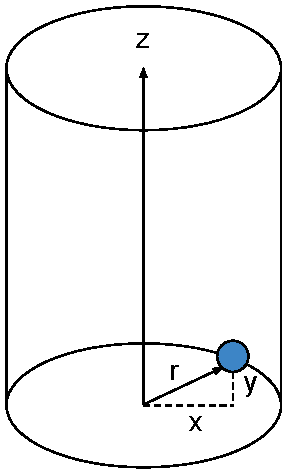
\includegraphics[width=0.2\textwidth]{cartesian_cylinder.pdf}
%  \caption{Using the nearest pore center as the origin, we represented the solute's
%  location along the pore axis in terms of the $z$ coordinates and their radial distance
%  from the pore centers in 2 dimensions, $x$ and $y$.}\label{fig:cartesian_cylinder}
%  \end{figure}
  
  We applied the IHMM to each of the 24 solute trajectories independently.
  Although the IHMM is capable of identifying an infinite number of states, 
  a Dirichlet process tends to exhibit a ``rich get richer" effect, favoring
  a fewer number of states. By applying the algorithm to each trajectory 
  independently, we reduce the possibility of lumping together multiple 
  similar states which we would prefer to stay separated before clustering.
  Note that the states identified by the IHMM are heavily influenced by 
  the Gaussian prior placed on $\mathbf{c}$ in Equation~\ref{eqn:var}. 
  In Section~\ref{S-section:prior_guesses} of the Supporting Information we outline our method for 
  choosing reliable prior parameters. The entries of $A$ and $\Sigma$ do 
  not vary over a wide range, so the final parameters were relatively insensitive
  to their priors.
  

  We ran 2000 iterations of the IHMM procedure in order to arrive at converged 
  state sequences and parameters for each state. Most parameters converged 
  quickly (within 50-100 iterations) while others took up to 1000 iterations.
  %BJC6: still need to make these figures.
  We defined the finalized parameters of each state as the average of the 
  parameters from each iteration recorded after the equilibration time point.
  We found the equilibration time point of each component of the $\mathbf{c}$ 
  vector as well as $A$ and $\Sigma$ matrices, and then used the longest 
  equilibration time of all dimensions as the equilibration time point.
  Further details are available in Section~\ref{S-section:convergence} of
  the Supporting Information.
  
  We reparameterized the time series, preserving the state sequence, in terms
  of the radial and axial coordinates ($r$, $z$) because $x$ and $y$ aren't 
  meaningful alone due to the system's radial symmetry. We converted the $x$ and 
  $y$ center-of-mass coordinates to $r$. We fixed the state sequence from the 
  3D parameterization and applied the inference component of the IHMM procedure
  to the cylindrical trajectories in order to estimate the VAR(1) parameters in
  terms of $r$ and $z$. Since we fixed the state sequence, and we are using conjugate
  priors, the VAR parameters converge very quickly (see Figure~\ref{S-fig:fixed_state_convergence}). Therefore, we only ran 
  the inference procedure for 100 iterations. 
  %However, note that the uncertainty in their
  %estimates are a function of the number of data points used in their estimate.
  
  We clustered like parameter sets in order to reduce the state space to
  a more easily interpretable size. For each solute studied, we identified 200-325
  independent states, each with separate VAR(1) parameters. Many of these states
  exhibit very similar dynamical behavior except their mean levels in $r$ and $z$
  are different.
  
  We reduced the parameter space used agglomerative clustering, a hierarchical
  clustering approach which uses a linkage criteria in order to successively merge
  similar clusters until a desired intracluster distance threshold or number of
  clusters is reached. We used the Ward linkage criteria, which works to minimize 
  the sum of the squared differences within all clusters.
    %MRS6: explain why Ward (make the cluster as minimally disperse?)
   	%BJC6: I'll add some plots to the SI and then write a better justification for
	% the paper. This is lower priority in mind for the thesis.
  We elected to choose the number of clusters rather than the distance threshold.
  For our data, non-parametric methods such as Bayesian Gaussian mixture models tend
  to delocalize the clusters in parameter space (see Section~\ref{S-section:agglomerative}
  of the Supporting Information).
  
  We clustered based on the two diagonal entries of $A$ and $\Sigma$ as well as the
  radial means, $\mu_r$, for a total of 5 variables. One can choose alternative clustering
  features, such as the eigenvalues of the $A$ and $\Sigma$ matrices, but we chose their 
  diagonals because they can be easily translated to solute behavior. The diagonals of $A$
  describe the correlation between sequential hops while the diagonals of $\Sigma$ describe
  the size of the hops in each dimension. We assume that cross correlations in the parameters
  are negligible for clustering.
   
  We also chose to cluster the diagonals of each matrix and the radial means
  independently before combining the clusters to assign final state labels. If we divide
  the total states into $m$ clusters based on the diagonal entries of $A$, $n$ more clusters 
  based on the diagonal entries of $\Sigma$, and $k$ clusters based on $\mu_r$, then there
  are a total of $mnk$ possible cluster combinations. This allows slightly more flexibility
  in the total number of states compared to clustering on all five features at once, since 
  there can be up to, but not necessarily exactly, $mnk$ states. 
  
  Choosing the number of clusters can be somewhat subjective so
  we attempted to add some structure to the selection process by following
  a set of qualitative and quantitative guidelines. We used the silhouette 
  test in order to score the quality of clustering as a function of the number 
  of clusters chosen. For our data, the silhouette test generally favors the 
  lowest number of clusters possible (see Section~\ref{S-section:nclusters} of
  the Supporting Information). However, choosing too few clusters tends to 
  not distinguish between visually obvious differences in 
  dynamic behavior. This results in finalized parameter sets that are averages of
  distinct behavior which presents further problems with the predictive modeling
  that we discuss later on. We aimed to maintain the highest silhouette score,
  and thus lowest number of clusters, possible while verifying that visually 
  distinct states stayed separated. Based on these guidelines, we decided to 
  group the $A$ and $\Sigma$ parameters into five clusters each and the radial
  means into three clusters. Of the 75 distinct states allowed by this formulation,
  the solutes in this study showed behavior from 32--36 distinct clusters. While
  this may seem like a high number of states, many are sampled infrequently.

  We remapped the state sequence based on the cluster assignments and generated a
  state transition probability matrix, $T$. The IHMM algorithm also produces an estimate
  of $T$, but since we fixed the state sequence, we decided to explicitly calculate $T$ 
  by counting the number of transitions between states compiled across all trajectories.

  We used the parameter inference component of the IHMM algorithm in order to 
  infer $A$ and $\Sigma$ of the clustered states.
   %BJC2: I'm unsure of the precise reasoning here.
  We could not simply take the mean of the clustered $A$ and $\mathbf{e}_t$ 
  parameters because it is not clear that this is a linear 
  operation for this problem. To circumvent this problem, we modified the ($r$,
  $z$) solute trajectories so that they had a mean of zero, leaving only the 
  fluctuations. We did this by the mean of each same-state segment of the 
  unclustered trajectory. We used the IHMM algorithm on this modified trajectory
  to infer the clustered state parameters by fixing the clustered state sequence. 
  
  We obtained $\mathbf{c}$ vectors of the clustered states by averaging 
  each value of $\mathbf{c}$ assigned to the same cluster. Note that we only care
  about the $r$ component of $\mathbf{c}$ because solute trajectories are not 
  bound in the $z$ direction.
  
  Finally, we generated stochastic trajectory realizations using the clustered
  parameter sets. We drew state sequences with transition probabilities given by
  $T$. While in a given state, we simulated motion according to the VAR(1)
  parameterization of that state. After each state transition, we reset the 
  unconditional mean of each state based on the particle's position immediately
  before the state transition occurred.
  
  \subsection{Tools for Exploring Mechanisms}\label{method:interactions}
  
  We determined the number of hydrogen bonds between each solute and the membrane
  as a function of time. Based on the geometric criteria of Luzar and Chandler, we 
  define a hydrogen bond to exist if the distance between donor, D, and acceptor, 
  A, atoms is less than 3.5\AA~and the angle formed by $D-H \cdots A$ is less than 
  $30\degree$.~\cite{luzar_effect_1996}
  
  We estimated the lifetime of hydrogen bonds by recording the length of 
  sequential frames where solutes remained hydrogen bonded. We still counted sequences
  where hydrogen bonds were broken for a single frame before reforming. Consistent
  with our previous work, we reported the 95th percentile of hydrogen bond lifetimes
  since their distribution is not Gaussian and to emphasize longer trapping periods. 
  
  We also measured the degree of association between solutes and sodium ions on a
  frame-by-frame basis. We define a sodium ion to be associated with an atom if they
  are within 2.5 \AA~of each other, as determined in our previous work.~\cite{coscia_chemically_2019}
  
  We developed a way to measure the local density of the membrane at arbitrary
  points in the unit cell. We histogrammed the positions in three dimensions
  Since our system is in a monoclinic unit cell, we periodically replicated
  the system in the +/- x, y and z directions and then chose the bounds on the
  histogram in order to create a rectangular box encompassing the unit cell with
  a 1 nm buffer between the histogram and unit cell boundaries. We then used a regular
  grid interpolator in order to allow interpolation at arbitrary points within the grid.
  
  We quantified solute motion using the time averaged mean squared displacement (MSD)
  of the solute center of mass trajectories. The time-averaged MSD measures all observed
  displacements over time lag $\tau$:
  \begin{equation}
  	\overline{z^2(\tau)} = \dfrac{1}{T - \tau}\int_{0}^{T - \tau} (z(t + \tau) - z(t))^2 dt
  \label{eqn:tamsd}
  \end{equation}
  where T is the length of the trajectory. We reported 1$\sigma$ confidence intervals 
  based on the results of 200 bootstrap trials. For each trail, we calculated the mean of 
  $n$ random trajectories chosen with replacement from the pool of trajectories, where 
  $n$ is the number of trajectories.

  \section{Results and Discussion}
  
  Solutes in this system show a wide range of behavior influenced by the 
  heterogeneity of the membrane's nanostructure as well as the interactions 
  between monomer and solute chemical functionality. Our application of the 
  IHMM can identify and distinguish these behaviors. The following approach 
  to analysis demonstrates how one can discover and explain the very complex
  behavior exhibited by solutes over long MD trajectories in terms of 
  solute-membrane interactions. Further, we can use the IHMM in order to generate
  stochastic trajectories, with dynamics similar to MD, so that we can estimate 
  macroscopic transport properties. 	

  \subsection{Automatic Detection of Distinct Dynamical Modes}\label{section:find_modes}
  
  We applied the IHMM to all trajectories of each of the four solutes studied.
  Based on our choice of clustering, we identified over 30 distinct dynamical
  modes for each solute. Many of these modes are sampled very infrequently and thus
  do not contribute significantly to a general understanding of solute transport behavior.
  In this section, we explore a subset of this data, focusing on the states
  and dominant interactions most common to solute trajectories.

  %MRS7: more descriptive title?  What about methanol?
  \subsubsection*{The Case of Methanol}
  
  %MRS6: likely just the summary of the methanol behavior should go in the main paper - the rest should be SI.
  Methanol exhibits a range of dynamic behavior. In Figure~\ref{fig:mechanism_map}, we
  plot a representative 2D methanol trajectory in cylindrical coordinates. The coordinates
  are colored according to the cluster with which methanol's dynamics are most consistent,
  which implies that this particular methanol trajectory exhibits 8 distinct dynamical 
  behaviors (in order of their first appearance, they are colored dark yellow, red, light
  blue, light green, orange, blue, teal and lime green). The solute time series are coupled
  with color coded bars which describe the solute's local environment and physical 
  interactions that it undergoes at that trajectory frame. From the top, they describe 
  whether the solute is associated with sodium, whether the solute is hydrogen bonding
  with the monomer as well as to what part of the monomer it is hydrogen bonding, and 
  finally, the local number density surrounding the solute. 

  \begin{figure}
  \centering
  \begin{subfigure}{0.75\textwidth}
  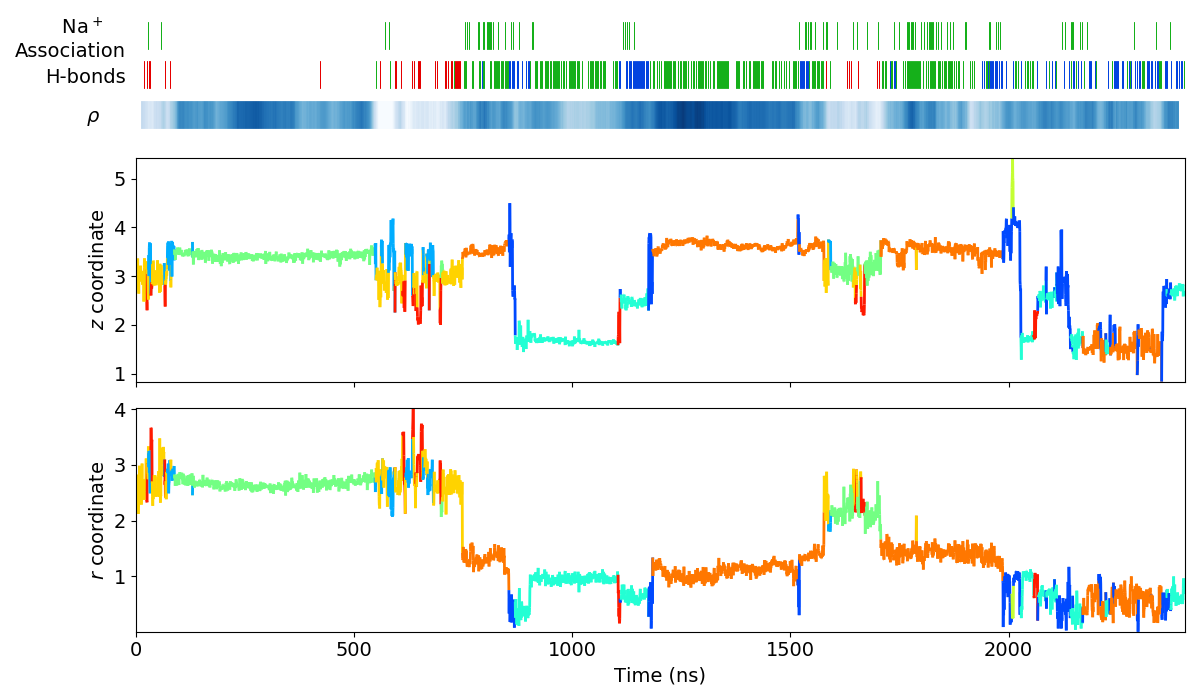
\includegraphics[width=\textwidth]{mechanism_map.png}
  \caption{}
  \end{subfigure}
  \begin{subfigure}{0.24\textwidth}
  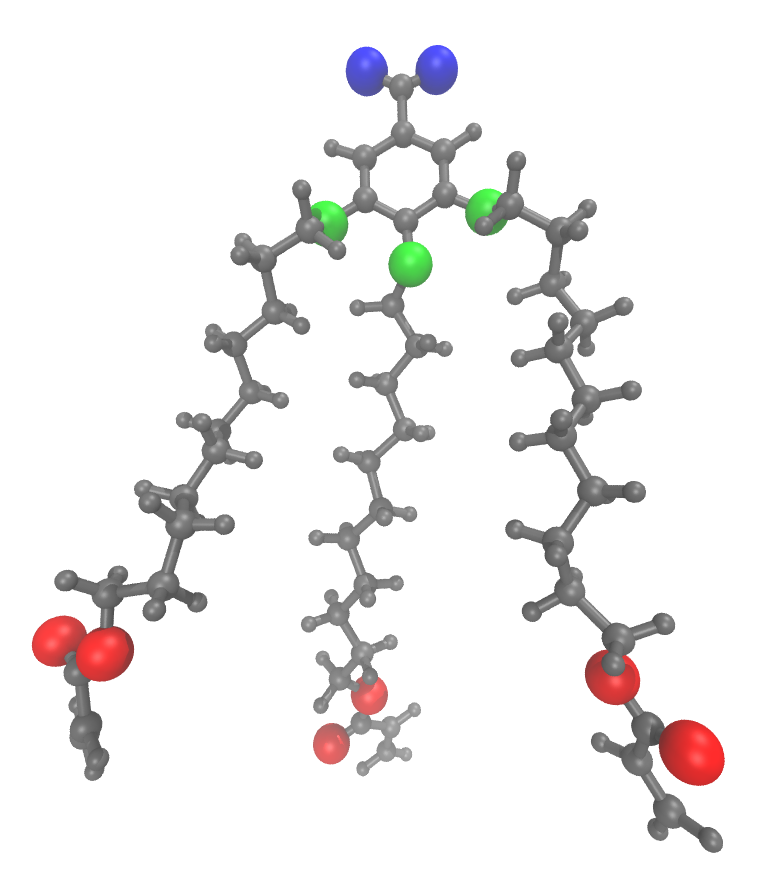
\includegraphics[width=\textwidth]{monomer_oxygens.png}
  \caption{}
  \end{subfigure}
  \caption{(a) We can learn a significant amount of detail about solute motion by viewing 
  solute trajectories color-coded according to their clustered dynamical behavior alongside
  plots of the dominant molecular interactions and descriptions of the membrane's local 
  environment. In the plot above, we show the radial and axial coordinates of a single
  methanol molecule over the course of the equilibrated portion of its MD simulation.
  Disjoint segments of the same color imply the solute behaves similarly at different 
  points of the trajectory because their VAR parameters place them in the same cluster. 
  There are eight distinct dynamical modes exhibited by this trajectory. In order
  of their first appearance, they are colored dark yellow, red, light blue, light green,
  orange, blue, teal and lime green. On the top of the plot are bars which represent different
  physical interactions and the membrane's local environment as a function of time. The top 
  bar is colored green at time points where solutes are associated with sodium. Methanol 
  associates with sodium ions relatively infrequently. The next bar down is colored when hydrogen
  bonds exist. The colors match the enlarged oxygen atoms highlighted in (b). Blue slivers
  correspond to hydrogen bonds donated to the monomer's carboxylate head group. Green slivers
  correspond to  hydrogen bonds donated to the ether linkages between the head groups
  and tails. Red slivers correspond to hydrogen bonds donated to the oxygens on the ends
  of the monomer tails. Methanol exhibits significant hydrogen bonding with all parts of
  the monomer. Which part of the monomer methanol hydrogen bonds to is heavily correlated
  to the solute's $r$ coordinate. Finally, the bar with the blue gradient represents the local 
  membrane density based on the solute's ($r$, $z$) coordinate. Darker shades of blue
  correspond to higher membrane densities. The density appears to be higher when methanol
  motion is restricted (e.g. from 75 to 550 ns). It is relatively low in areas where methanol's
  position fluctuates significantly (e.g. from 550 to 700 ns). 
  }\label{fig:mechanism_map}
  \end{figure}

  One can gain useful chemical intuition just by studying plots like
  Figure~\ref{fig:mechanism_map}. It is clear that, for methanol, association 
  with sodium is a much rarer interaction than hydrogen bonding with the 
  LLC monomers. Methanol hydrogen bonds to all regions of the monomers dependent
  on its radial position. Its fluctuations tend to be smallest when hydrogen bonded
  or in areas of high local number density. For example, from approximately 75 to 
  525 ns, methanol appears to be trapped in a high density region of the tails.
  In the time that follows, it enters a region of relatively low density where 
  fluctuations are quite large. During this time period, there is intermittent, 
  short-lived hydrogen bonding with the oxygen atoms at the tail ends, as suggested
  by the frequent state changes during that time period and red slivers in the bar
  above. Significant hops in the $z$ direction appear to be described by the dark blue
  state. After entering the dark blue state ca. 850 ns, methanol appears to jump
  significantly in the $z$ direction from a hydrogen bonded state with the ether 
  linkages to a hydrogen bonded state with a head group in a monomer below it.

  It is clear that there is a wealth of information in these plots, but they don't give
  the complete picture needed in order to formulate LLC membrane design principles. One
  can analyze each segment sequentially and form a clear picture of this instance of 
  methanol's behavior without the need to visualize the trajectory with software like VMD.
  However, it is still possible to gain a more general understanding of methanol's average
  behavior.
  
  %BJC: I'm not sure whether to spell out the numbers or not. 'six state' versus '6 states'; 'eight out of 24' or '8 out of 24'
  % 'State one or State 1' 
  We may learn the most by studying the dynamical modes common to the majority of 
  the solute trajectories. Using the IHMM, we identified 33 total dynamical modes 
  exhibited by methanol. Of those, only six states appear in a third (8 out of 24) 
  or more methanol trajectories, and three of them appear in over 50 \% of the 
  methanol trajectories. 12 of the detected states are shared by two or less 
  methanol trajectories. In Figure~\ref{fig:common_states_MET_lines}, we plot 
  representative dynamics of each of the six states which we determined to be prevalent.
  We also chose to study a seventh state, which only appears in three out of
  24 trajectories, because methanol experiences very long periods of entrapment
  while in this state. Long trapping events, even if they are relatively rare, will
  have a significant influence on solute flux. No trajectory contains all seven states.
  However, the trajectory in Figure~\ref{fig:mechanism_map} exhibits all modes except
  states 6 and 7. The states in Figure~\ref{fig:common_states_MET} are colored to match
  states that also appear in Figure~\ref{fig:mechanism_map}.
    
  We can begin to dissect the dynamics of each state by studying their parameters.
  States 1, 3 and 5 have radial means near 1 nm or less (see y axis of $r$ direction 
  plot in Figure~\ref{fig:common_states_MET_lines}), which suggest that they occur
  close to the pore centers. States 2, 4, 6 and 7 occur well within the tail region
  of the membrane. States 1 and 2 have higher covariances in both the axial and radial
  directions compared to all other states. Covariance in each dimension appears to have
  a strong correlation. States 3 and 5 (in the pore region) as well as states 4, 6 and
  7 (in the tail region) are primarily distinguished based on their autoregressive 
  coefficients, A. Higher values of A generally lead to more wandering about the state
  mean. One could argue that the parameters of states 3--7 are actually very close which
  suggests that solutes might behave alike in topologically distinct regions of the 
  membrane.

  Despite some similarity in their VAR parameters, the length of time spent in states 
  3--7 appears to be dependent on the solute's radial location. Based on the 
  self-transition probabilities, we estimated the average time spent by each solute in
  each state (Figure~\ref{fig:dwell_times_MET}). States 3, 5 and 7 have long dwell times
  relative to the rest because they have high self-transition probabilities. Somewhat 
  surprisingly, both states 3 and 5 correspond to solutes located close to a pore center,
  where one might expect solute motion to be less restricted. Although solutes in states
  4 and 6 are in the viscous tail region, their dwell times are only intermediate. This
  could be due to inhomogeneity in the tail region which causes transitions between many
  different trapped states but with little net effect on solute MSD. However, there are
  instances of states within the tail region with dwell times that exceed 100--200 ns,
  as shown by our inclusion of state 7. There are no other states with dwell times longer
  than state 5 in the pore region.
  
  States 1 and 2 exhibit the shortest dwell times of the states studied. This is 
  consistent with the trajectory in Figure~\ref{fig:mechanism_map}. State 2 is the 
  shortest lived state, appearing to bridge other tail region states. State 1 
  appears to represent a significant hopping state. It has a high covariance and
  occurs near the pore center, where there is less obstruction to solute motion.
  It's dwell time of ca.~8 ns, suggests that solutes stay in this highly mobile 
  state for long enough for their positions to displace significantly.
  
  \begin{figure}
  \centering
  \begin{subfigure}{0.6\textwidth}
  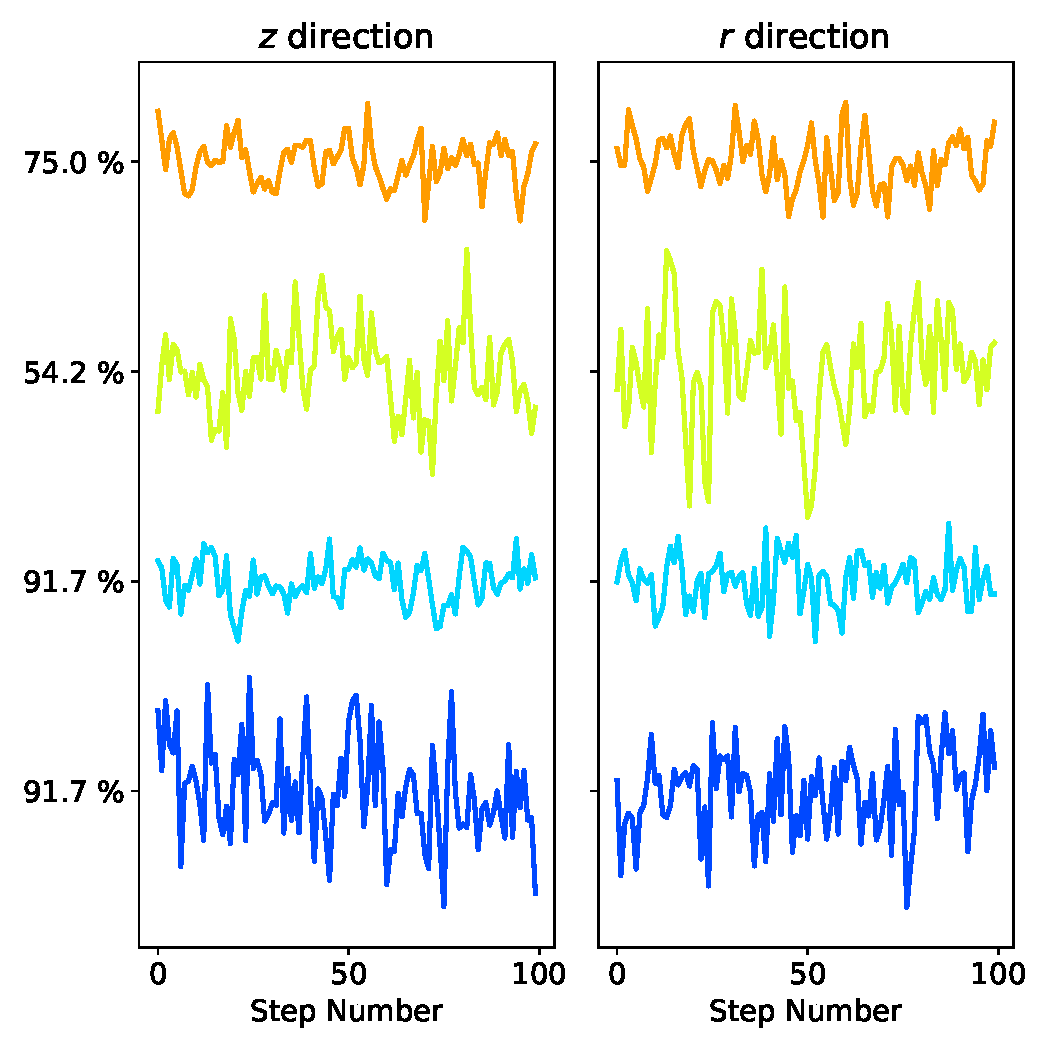
\includegraphics[width=\textwidth]{common_states_MET.pdf}
  \caption{}\label{fig:common_states_MET_lines}
  \end{subfigure}
  \begin{subfigure}{0.35\textwidth}
  % BJC: I'll bootstrap some error bars on this by drawing the transition probabilities 
  % from a Dirichlet distribution.
  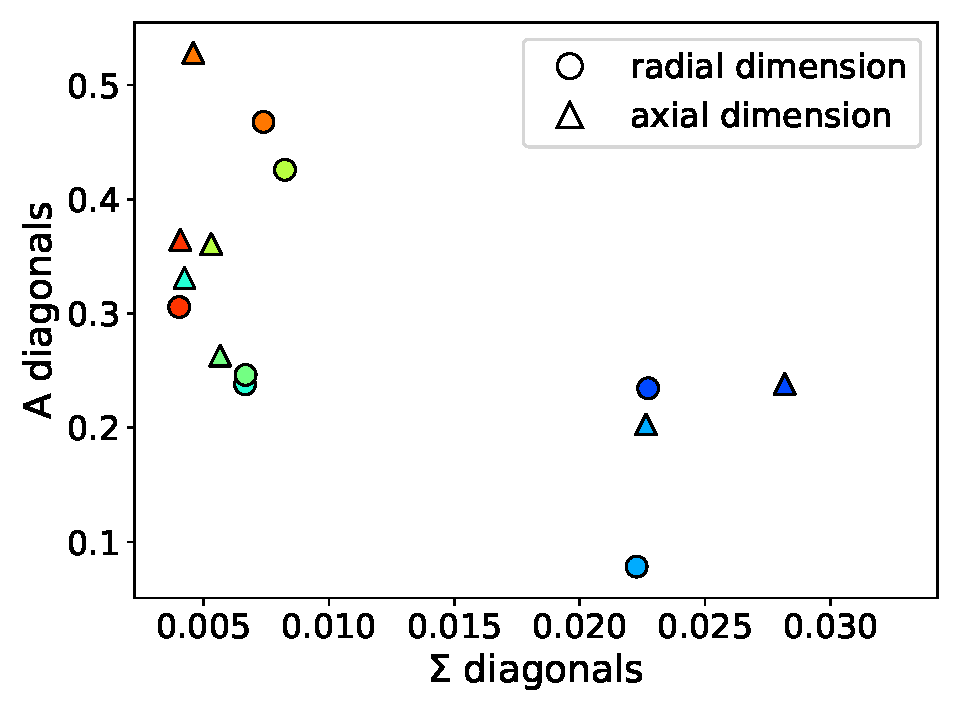
\includegraphics[width=\textwidth]{A_sigma_scatter_MET.pdf}
  \caption{}\label{fig:A_sigma_scatter_MET}
  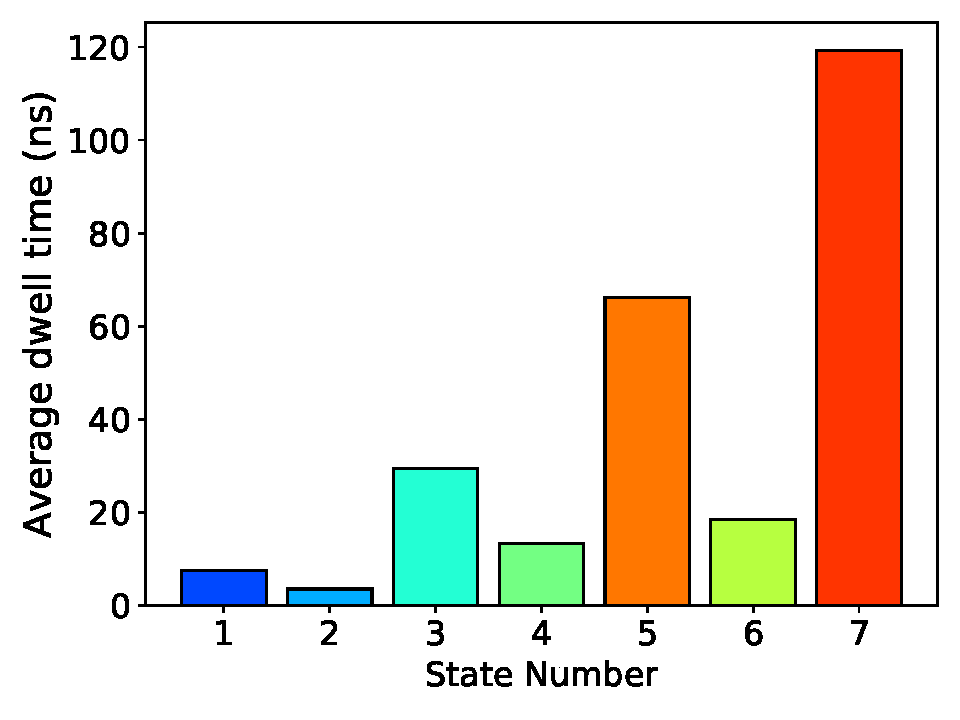
\includegraphics[width=\textwidth]{dwell_times_MET.pdf}  %BJC5: maybe better as 95 % confidence rather than mean
  \caption{}\label{fig:dwell_times_MET}
  \end{subfigure}
  \caption{We can learn the most about methanol's behavior by studying the dynamics
  of the states common to many of the methanol trajectories. In (a), we show representative
  dynamics of six states that are common to more than one third of the solute trajectories. 
  The $y$-axis labels of the $r$ coordinate plot specify the radial mean of each clustered 
  state. 
  %MRS7: it's confusing to have the R not in order of r. Emphasize this more in the caption, maybe think of something a bit different for the final paper. Reads odd to have numbers not in order along an axis.
The percentage of trajectories in which the states appear are labeled to the right of
  the $r$ plots. States 1--5 appear in the trajectory shown in Figure~\ref{fig:mechanism_map}
  and are colored to match for easy visual comparison. All time series have a mean of zero and are
  shifted to put the mean in line with the $y$-axis labels for the purpose of visualizing them. 
  (b) We can begin to understand the solute behaviors demonstrated in (a) by understanding their VAR 
  parameters. States 1 and 2 have higher covariances in both the axial and radial directions compared
  to all other states. This should lead to significant solute displacement. Covariance in each dimension
  appears to have a strong correlation. States 3--6 all have relatively low covariances, which may
  be characteristic of trapped states. They are primarily distinguished based on the magnitude of their 
  autoregressive coefficients, A, and radial means. Higher values of A imply motion which wanders 
  more about the mean. States 1, 3 and 5 have radial means near 1 nm or less, which suggest that they
  occur close to the pore centers. States 2, 4 and 6 occur well within the tail region of the membrane.
  (c) Using the transition probabilities (p), we estimated the average time spent within each 
  of the states using 1000 simulations of a Bernoulli process where we continued to draw until transitioning
  out of the state with probability 1 - p. Of the prevalent states, states 1 and 
  2 exhibit the shortest dwell times alongside their high covariances. States 5 and 7 have the longest dwell times in the pore and tail regions respectively.
  }\label{fig:common_states_MET}
  \end{figure}
  
  Most of what we have learned thus far has been based on the parameters of our
  model with some qualitative validation using a single methanol trajectory. While 
  we may be able to further corroborate our arguments by analyzing more
  individual trajectories, it is more useful to correlate the state behavior with
  solute-membrane interactions.

  The types of hydrogen bonding undergone by solutes is dependent on radial
  location (see Figure~\ref{fig:hbond_pichart}). States with radial means near 1 nm
  or less (states 1, 3 and 5) typically hydrogen bond with the monomer carboxylate
  groups and ether linkages. States with radial means greater than 1 nm (states 2,
  4, 6 and 7) tend to hydrogen bond with the monomer tails. In the past we've shown
  that there is a gradual transition from the hydrophilic to hydrophobic region in
  these membranes, meaning the monomer location is not tightly bound in $r$. Therefore,
  there are instances of hydrogen bond interactions that one might consider 
  uncharacteristic based on the state's radial mean.
  
  States which exhibit longer dwell times have longer hydrogen bond lifetimes (see
  Figure~\ref{fig:hbond_pichart}). States 3--7 have significantly longer hydrogen 
  bond lifetimes than states 1 and 2. It makes physical and mathematical sense that
  states 1 and 2 should not stay trapped by hydrogen bonding for long periods because
  they typically take large hops as communicated by their large covariances.
  In the tail states, hydrogen bond lifetimes appear to increase with their dwell 
  times. However, in the pores, the same linear relationship does not hold.
  For example, state 5 has the lowest hydrogen bond lifetime of states 3--7
  despite having the second longest dwell times. 
  
  The local density experienced by solutes may have an impact on the length of solute 
  entrapment. On average, solutes in state 5 are surrounded by a relatively high density
  of particles. Based on its radial location and preference towards hydrogen bonding
  with the ether linkages (see Figure~\ref{fig:hbond_pi_charts}), it is reasonable to
  assume that while in state 5, methanol spends most of its time just outside the 
  pore region, sandwiched between the monomer head groups. Although state 5 hydrogen
  bonds break more frequently than one might expect for a state with long dwell times,
  it is possible that the solute's dense surroundings prevent it from wandering off 
  before the hydrogen bonding interaction can be recovered. This may explain the 
  behavior of the methanol in state 5 of the trajectory in Figure~\ref{fig:mechanism_map}
  where the solute's center of mass appears to move more freely about its mean than 
  other trapped states. The data suggests that methanol molecules in state 3 lie closer
  to the pore center than state 5 because they tend to hydrogen bond most frequently 
  with the carboxylate groups. Methanol molecules which experience state 3 are subject 
  to a lower density local environment and rely more heavily on hydrogen bonding interactions, 
  evidenced by their longer lifetimes, to stay trapped.
  
  States describing behavior in the tail region show a direct relationship between 
  hydrogen bond lifetimes and local density. Methanol molecules which experience state 2 
  spend their time in a low density region of the tails where they can easily break free
  of hydrogen bonds. Conversely, methanol molecules trapped in state 7 are in the densest 
  region of all states studied. It is likely difficult for methanol to escape these high 
  density regions and its position is further stabilized via hydrogen bonding.
  
  %BJC4: I didn't put sodium ion association in this figure because it's infrequent. 
  %BJC4: If I compare to acetic acid or urea, I could add it back. I was thinking of splitting
  % the pi chart in half with slices corresponding to hbonds on one side and association on the other
  \begin{figure}
  \centering
  \begin{subfigure}{0.54\textwidth}
  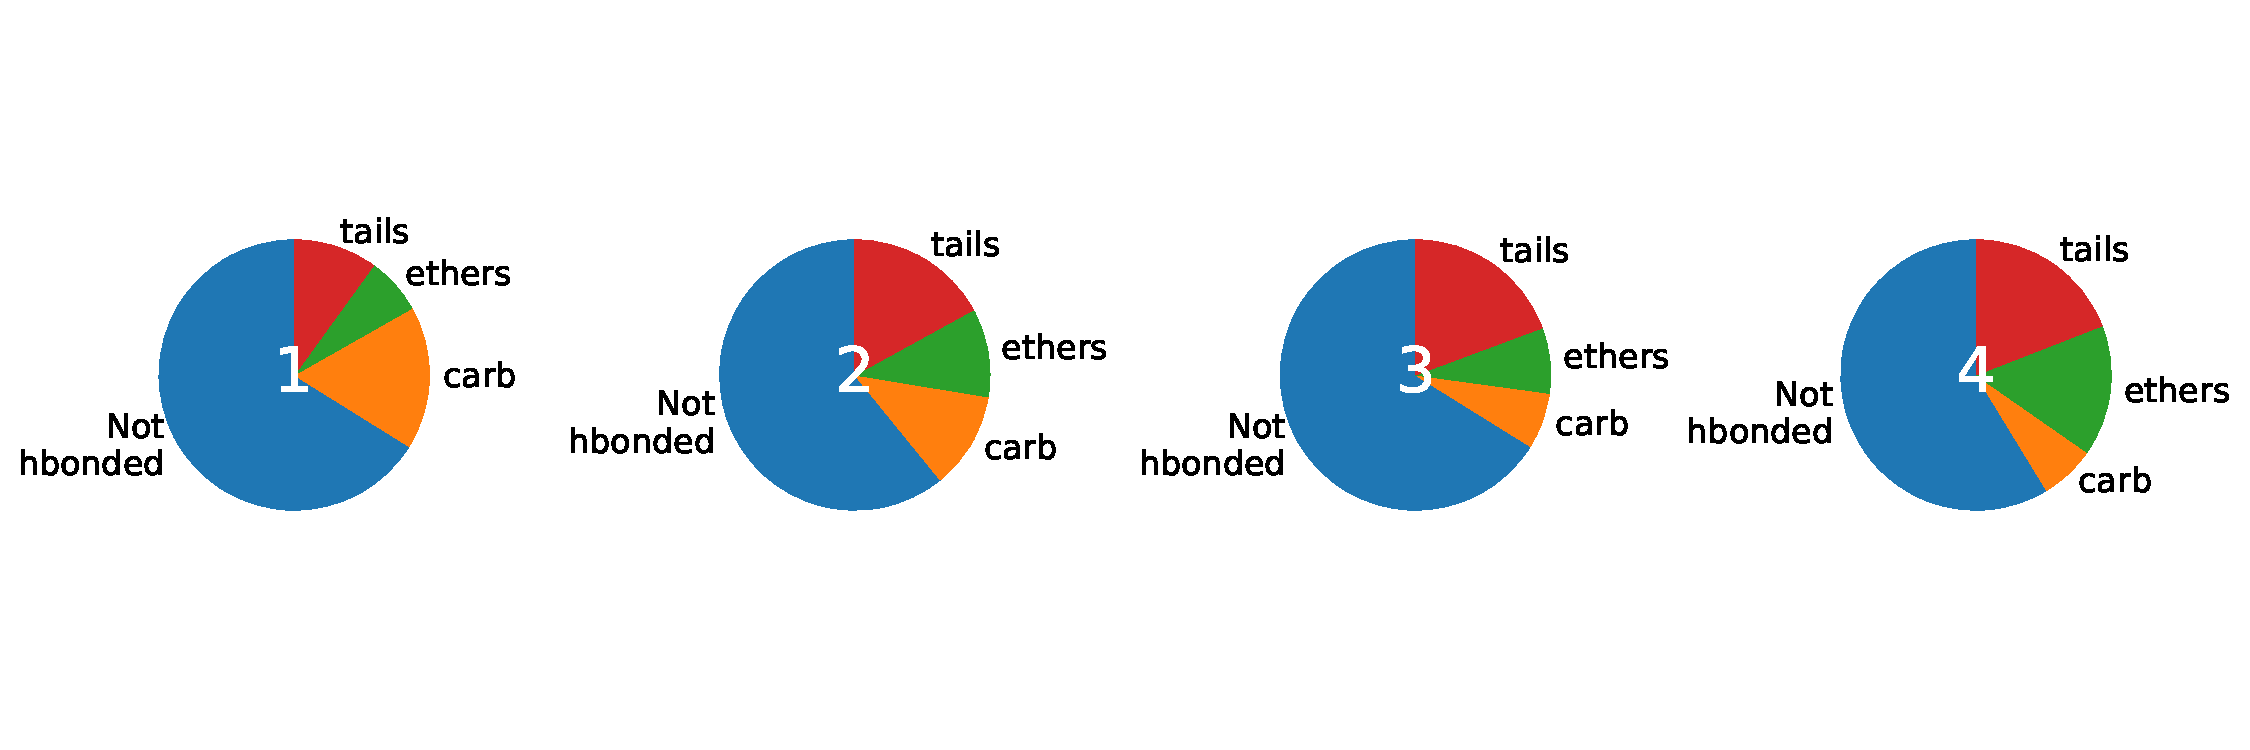
\includegraphics[width=\textwidth]{hbond_pi_charts.pdf}
  \caption{}\label{fig:hbond_pi_charts}
  \end{subfigure}
  \begin{subfigure}{0.45\textwidth}
  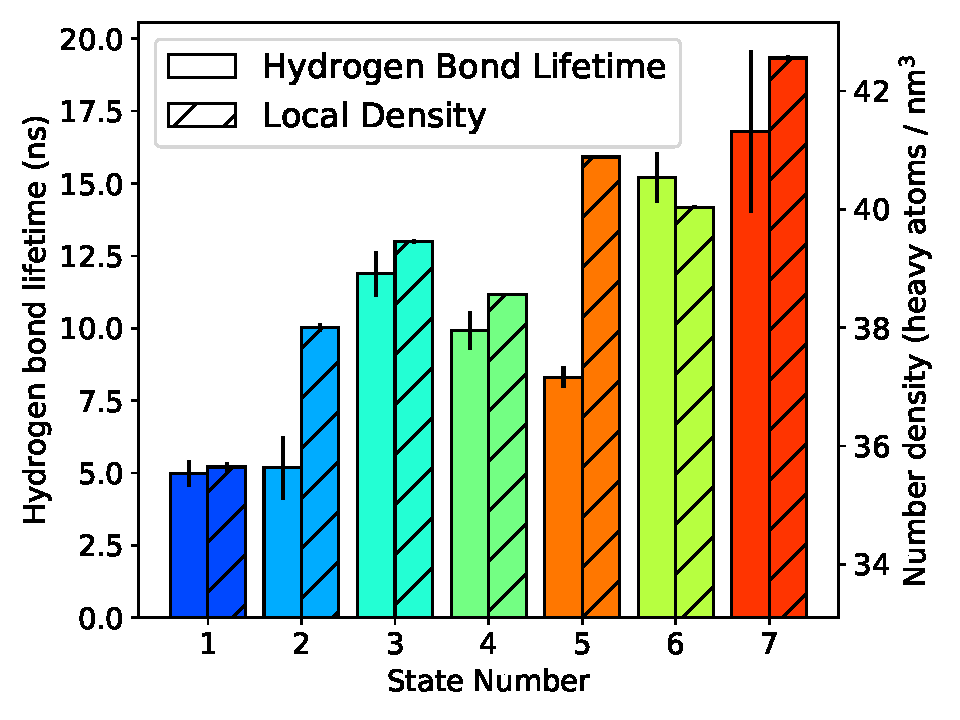
\includegraphics[width=\textwidth]{hbond_lifetimes_density_MET.pdf}
  \caption{}\label{fig:hbond_lifetimes_density_MET}
  \end{subfigure}
  %MRS7: should it be ``methanol hydrogen bonding in different segments''? 
  \caption{(a) Methanol hydrogen bonds with different segments of the LLC monomer
    %MRS7: why are some wedges bigger? (green on 2 and 6 for example)
  dependent on the state. States with mean radial locations in the pore region tend to
  hydrogen bond with the head groups and ether linkages. States with mean radial
  locations in the tails tend to hydrogen bond with the tail oxygen atoms.
  (b) Hydrogen bond lifetimes and the local density experienced by methanol
  molecules can help us to understand dynamical states in terms of membrane 
  interactions. States 1 and 2, which have large covariances, also have short
  hydrogen bond lifetimes and exist in relatively low density regions. The
  hydrogen bond lifetimes of methanol in states with radial means in the tail
  region tend to increase with local density and mean dwell times. 
  %MRS7: not clear from graphic which ones are in the pore.
  %MRS7: is there any legend for the color for b? If same as above figure, indicate. Don't REALLY need color since they bars are already labeled, so it's 2 sources of duplicate information.
  %MRS7: cross-hatching doesn't appear in the legend? Not sure which is which (I assume hatched is number density because closer to that axis).
  This monotonic
  relationship does not exist for states in the pore region. The high 
  local density experienced by state 5 methanol molecules may explain why 
  hydrogen bond lifetimes are short but dwell times are high. State 5 methanol's
  preference towards hydrogen bonds with ether linkages suggests that the solute
  sits between LLC monomer head group which prevent it from wandering to far
  before recovering its previous hydrogen bond.
  }\label{fig:hbond_pichart}
  \end{figure}
  
  % BJC5: I think I want to do an abbreviated study here on acetic acid or urea 
  % since it will incorporate sodium ion association. 
  
  \subsubsection*{Behavior of Other Solutes}
  
  We applied the IHMM to the other three solutes in this study: urea, acetic acid
  and ethylene glycol. 
  \begin{itemize}  
    \item Not only can we use the model to study the dynamics of each solute 
    individually, but we can compare their behavior in order to improve our
    understanding of more subtle mechanistic details.
  \end{itemize} 
  
  The size and chemical functionality of the solutes dictates the interactions which
  influence solute transport. 
  \begin{itemize}  
    \item In Figure~\ref{fig:hbonds_assoc_summary}, we show that the solutes 
    donate hydrogen bonds and associate with sodium ions to varying degrees.
    \item We also show the solute MSDs after a 1000 ns time lag. 
    \item It is not immediately obvious why the MSDs follow this trend.
    \item The states identified by the IHMM can help us shed some light.
  \end{itemize}
  
  \begin{figure}
  \centering
  \begin{subfigure}{0.45\textwidth}
  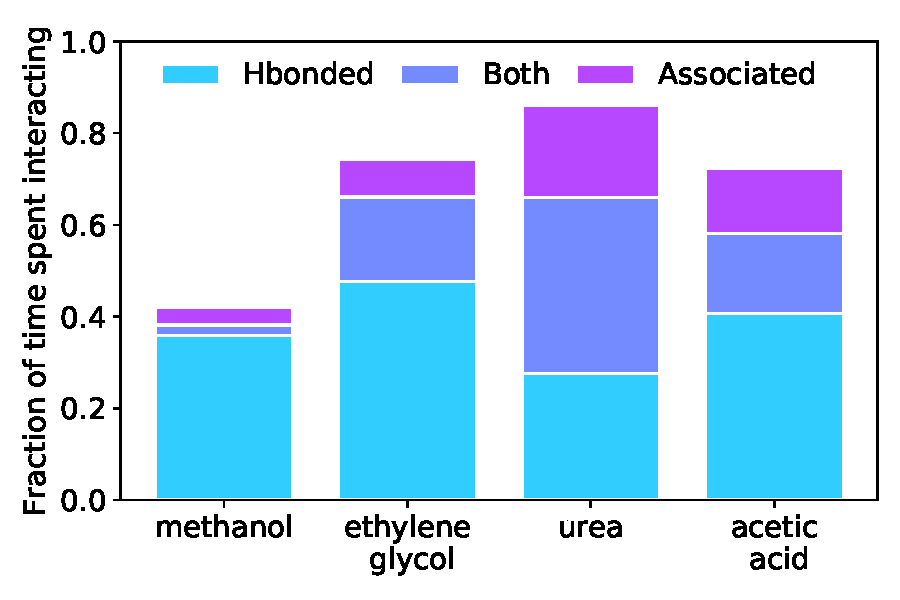
\includegraphics[width=\textwidth]{hbonds_assoc_summary.pdf}
  \caption{}\label{fig:hbonds_assoc_summary}
  \end{subfigure}
  \begin{subfigure}{0.45\textwidth}
  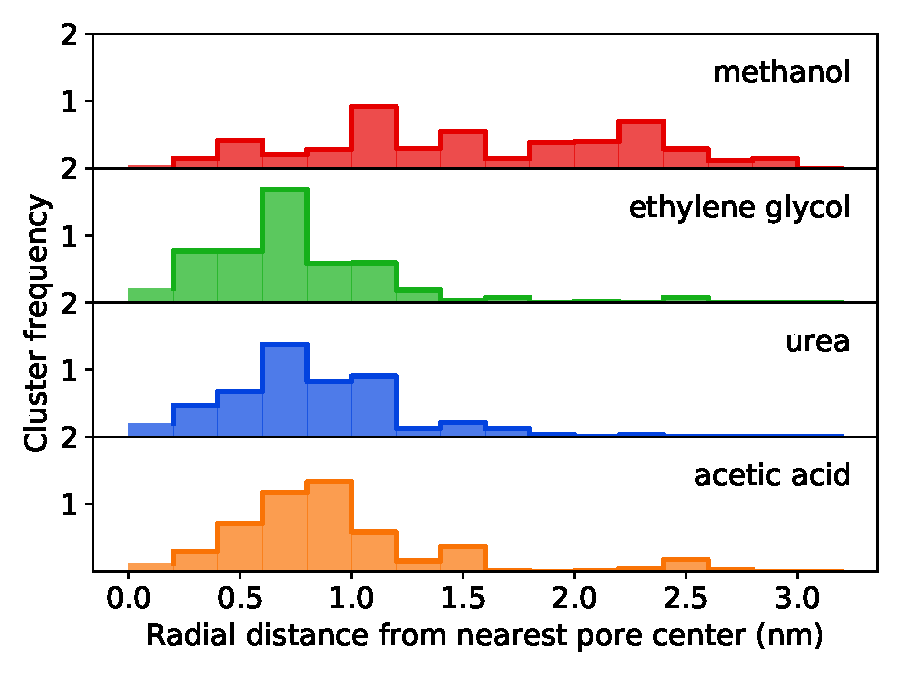
\includegraphics[width=\textwidth]{rdf_summary.pdf}
  \caption{}\label{fig:rdf_summary}
  \end{subfigure}
  \begin{subfigure}{0.45\textwidth}
  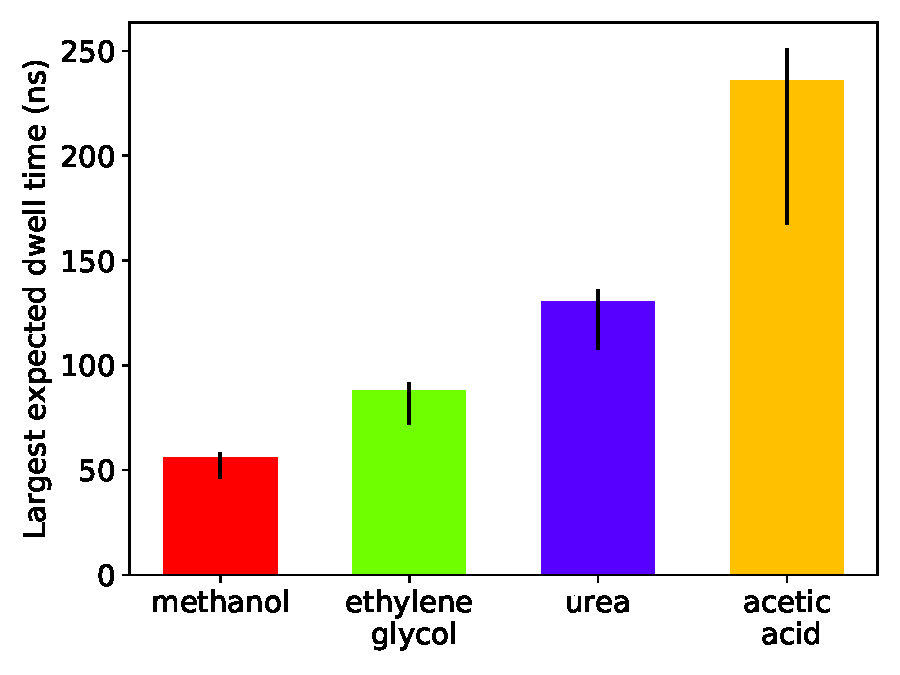
\includegraphics[width=\textwidth]{dwell_time_summary.pdf}
  \caption{}\label{fig:dwell_time_summary}
  \end{subfigure}
  %MRS7: maybe in dwell time legend, say ``Max dwell in'' instead of ``Max of''
  \begin{subfigure}{0.45\textwidth}
  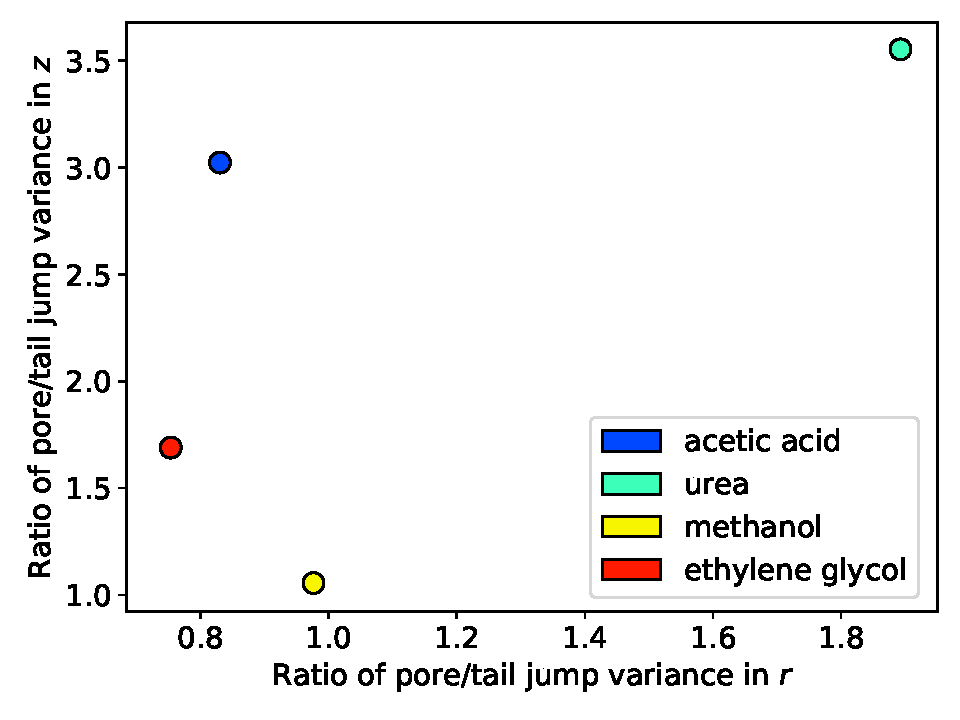
\includegraphics[width=\textwidth]{cov_summary.pdf}
  \caption{}\label{fig:cov_summary}
  \end{subfigure}
  %MRS7: is c) methanol?  I thought it wasn't associating with Na+ much.
  %MRS7: methanol yellow is hard to see in c)
  \caption{(a) Solutes hydrogen bond and associate with sodium ions
  to different degrees. Sometimes, they participate in both interactions at
  once. The frequency at which solutes interact via either mechanism does
  not appear to be linearly related to the solute's mean squared displacement
  after a 1000 ns time lag. (b) We histogrammed the means of the clusters weighted
  by the number of 
  %MRS7: ``transitions out'' instead of emisssions?
  emissions from that cluster. Most solutes spend the majority of
  their time close to the pore center. Only methanol has a significant peak
  beyond 1.5 nm from the pore center. (c) The trend in the maximum dwell time
  among prevalent states for each solute is inversely related to the
  solute's MSD. In some cases, non-prevalent states show very long dwell times,
  which may have a significant impact on solute MSD. (d) All solutes tend to
  take larger hops in the $z$ direction when they are in the pore versus in 
  the tails. All solutes except urea make slightly larger radial hops while 
  in the tails.
  %BJC6: I made this plot out of curiosity, not sure if I'll use it yet.
  }\label{fig:summaries}
  \end{figure}
  
  Hydrogen bonding and sodium ion association interactions are far more 
  common when solutes stay near the pore centers.
  \begin{itemize}
    \item In Figure~\ref{fig:rdf_summary}, we plot the distribution of the 
    radial means of each cluster weighted by the time spent in that cluster.
    \item All solutes except methanol spend the majority of their time near
    the pore centers (roughly defined as within 1.5 nm).
    \item As we showed earlier, methanol spends a significant portion of its
    time trapped in the dense tails.
  \end{itemize}
  
  % BJC: we can probably use this to create a new definition of the pore and tail region.
  % and perhaps focus on transitions between them.
  Solute size likely has a large effect on their preferred radial location within
  the pores.
  \begin{itemize}
    \item The histograms in Figure~\ref{fig:rdf_summary} have a clear vacancy between
    what one might consider the pore and tail region, most evident in methanol's 
    distribution of radial positions.
    \item The area between the head groups and the distal regions of the tails is
    dense and hydrophobic which creates a considerable energy barrier to be overcome
    in order to transition to that region.
    %BJC: I wonder if there is a state which corresponds to the jump from pore to tail region. Might be hard to pick up.
    \item Methanol is the smallest solute in this study and therefore appears to 
    have the easiest time crossing into the tails. 
  \end{itemize}

  Despite their close proximity to the low density aqueous pore region, acetic
  acid, ethylene glycol and urea exhibit a range of trapping behavior.
  \begin{itemize}
    \item It is clear that the number of polar interactions is not directly
    related to solute MSD. Acetic acid participates in a similar number of 
    interactions relative to urea and ethylene glycol, but its MSD is considerably
    lower.
    \item For the purpose of this analysis, as in the previous section, we 
    defined states that appear in more than one third of the trajectories to
    be prevalent states.
    \item In Figure~\ref{fig:dwell_time_summary}, we plot the longest dwell
    times exhibited by each solute among the prevalent states as well 
    as out of all the states.
    \item The state which exhibits the longest dwell times among all acetic
    acid states appears in 9 different trajectories, making it a prevalent state,
    and occurs 1 nm from the pore center. %BJC: check exact radius
    \item Although urea possesses the state with the longest dwell time among the
    solutes studied, it occurs in the tail region with prevalent states having 
    much shorter dwell times.  %BJC: get radius of long entrapment.
    \item Ethylene glycol appears to be the least subject to trapping.
  \end{itemize}

%  The combination of a carbonyl group, which binds strongly to sodium, and a 
%  hydroxyl group, which can form strong hydrogen bonds, makes acetic acid
%  particularly prone to trapping.
%  BJC6: more complicated than this. I will revisit.

  \subsection{Reproducing MD Trajectories and MSDs with the IHMM}
  
  %BJC5: something we can do for the supporting information to show that this approach is valid: Eliminate nonidealities in our MD trajectories (compared to a pure VAR process) and use toy data to generate trajectories based on some number of states with different parameters. Generate an MSD with those. See if we can reproduce with our model. Can also use this to test new strategies.
  %MRS6: toy data is actually a VERY good idea.  Use a VAR process that looks like MD, and then try to cluster it, and figure out why different.  
  
  We can use the IHMM in order to generate stochastic trajectory realizations
  which bear some qualitatively similar characteristics to those output
  by our MD simulations. Because we clustered the data, we are left with a 
  single transition probability matrix which allows transitions between dynamical
  behaviors shared by the 24 MD trajectories. In 
  Figure~\ref{fig:trajectory_realizations_MET}, we show some stochastic realizations
  generated by our models compared directly to MD. The trajectories show clear 
  periods of entrapment with intermittent hops.
  
  %BJC5: the goal is to figure out how to fix this for the paper.
  %BJC5: this is more of a 'how can this be improved' section for the dissertation.
  %MRS6: got it.
  The MD trajectories show much broader variability in their overall motion than realizations
  of the IHMM model. 
  %MRS6: definitely an important point for the paper: clustering things together might make trajectories too typical.
  Some trajectories span a wide range of $z$ coordinates, while others stay
  trapped for nearly the entire simulation. Our model is very unlikely to generate 
  trajectories with dwell times similar to the third MD trajectory shown in 
  Figure~\ref{fig:trajectory_realizations_MET}. This is because the realizations 
  generated by our model are representative of the average behavior of solutes studied.
  It is possible that certain states with long dwell times should have been
  clustered as their own, but the transition probabilities would have high uncertainties.
        %MRS6: is it necessarily a problem that the transition probabilities have high uncertainties? If one is drawing from the Dirichlet distribution, uncertainty isn't a big deal. The trapping just doesn't quite seem to be as long as MD.
        %MRS6: the other issue is apparent suppression on variance in the jumps, but that may be harder to get. 
  It is also possible that we should not be using a static transition matrix in 
  order to generate stochastic trajectories, but rather sample the rows of the transition
  matrix from a Dirichlet distribution since average dwell times are highly sensitive to
  self transition probabilities.
        %MRS6: right uncertainty matters less here.
  %BJC5: maybe a figure showing the MSDs of all the MD trajectories versus a subset of 
  % stochastically generated trajectories. I image the stochastic ones will have a much
  % tighter distribution.

  \begin{figure}
  \centering
  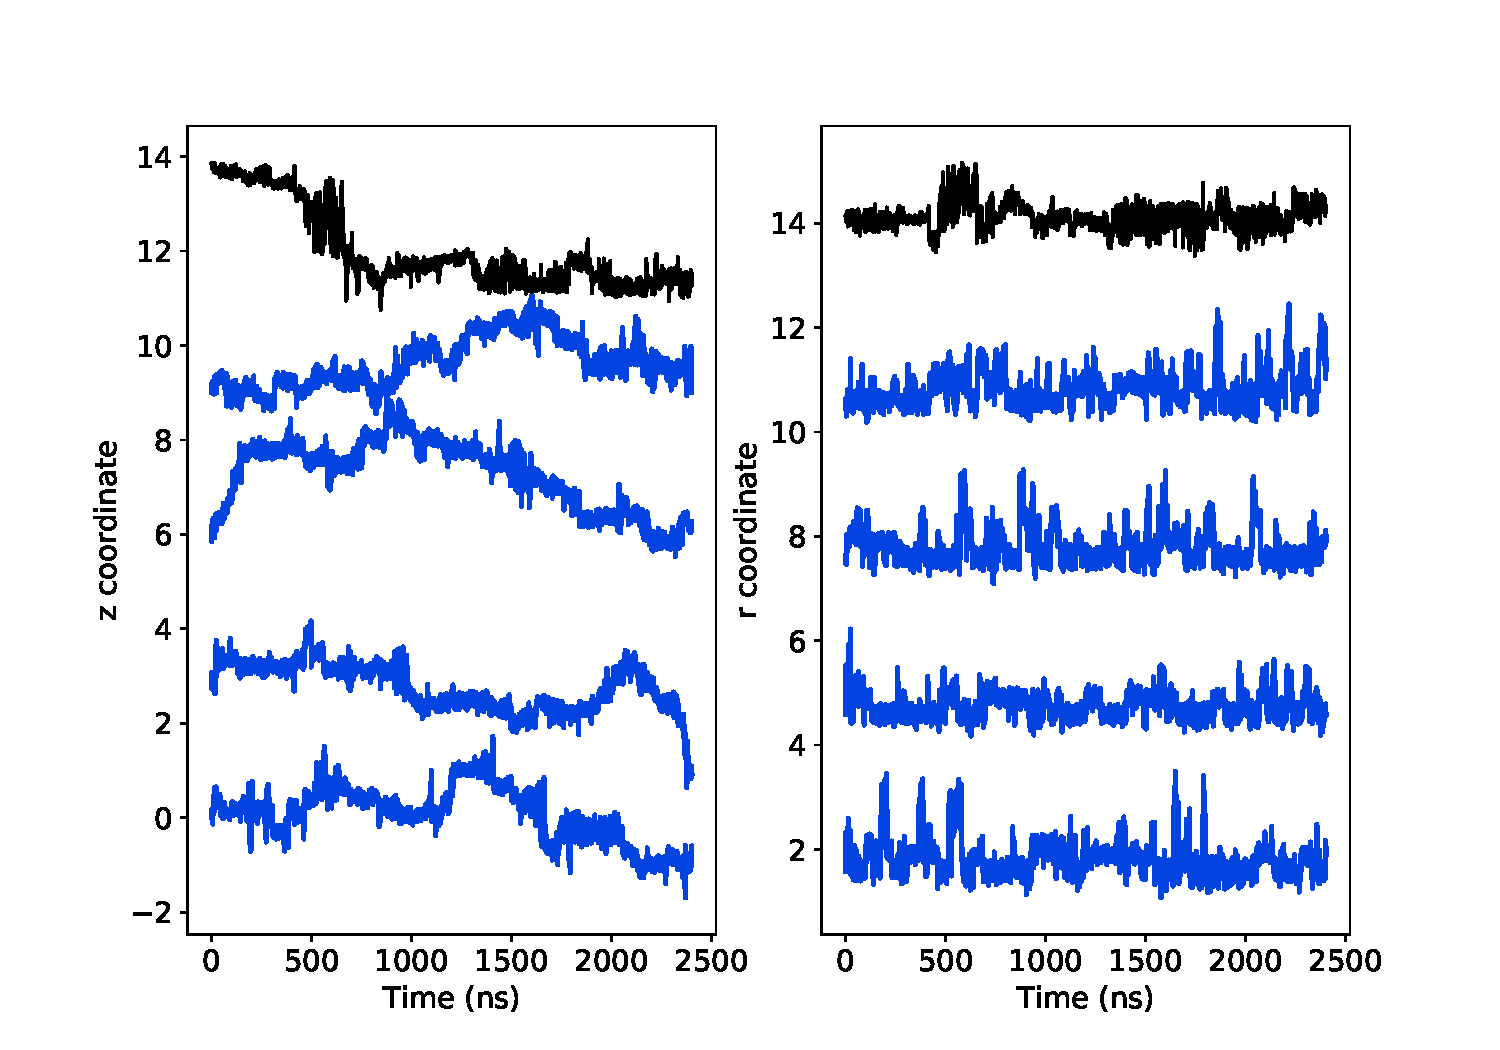
\includegraphics[width=\textwidth]{trajectory_realizations_MET.pdf}
  %MRS5: maybe it would be good to put a dotted line through each of the centers of the offset trajectories?
  %BJC5: TODO: redo these plots with r clusters
  %MRS7: still odd it doesn't stay at large r.
  %MRS7: can you restart the radial coordiante, so 0-3 just repeats, instead of going up tp 17.5?
 \caption{We can generate trajectories which bear some qualitative resemblance to the MD 
  trajectories. Solute trajectories generated by our model (blue) show the same
  hopping and trapping behavior exhibited by MD (black). The behavior of individual 
  MD trajectories tend to show wider variability than our model's realization because
  the model effectively represents the average behavior of the MD trajectories. This 
  implies that much longer simulations or a different method of trajectory generation might
  be necessary in order to obtain stochastic realizations with the same range of behavior
  as MD.
   }\label{fig:trajectory_realizations_MET}
  \end{figure}
  
  The MSDs calculated by stochastic realizations of our model are quantitatively similar to
  MD. For all solutes except acetic acid, our predicted MSD curve lie close to but below the
  1$\sigma$ confidence intervals of MD. However, in these cases, the average MD MSDs are 
  driven up by single trajectories with uncharacteristically large MSDs. It is possible that
  an improved trajectory generation approach may allow for this highly variable behavior.
  If we remove these uncharacteristic trajectories, the agreement between MD and our realizations
  improves. Acetic acid has no obvious outliers and shows good agreement between MD and
  IHMM realizations.
  
  \begin{figure}
  \centering
  \begin{subfigure}{0.45\textwidth}
  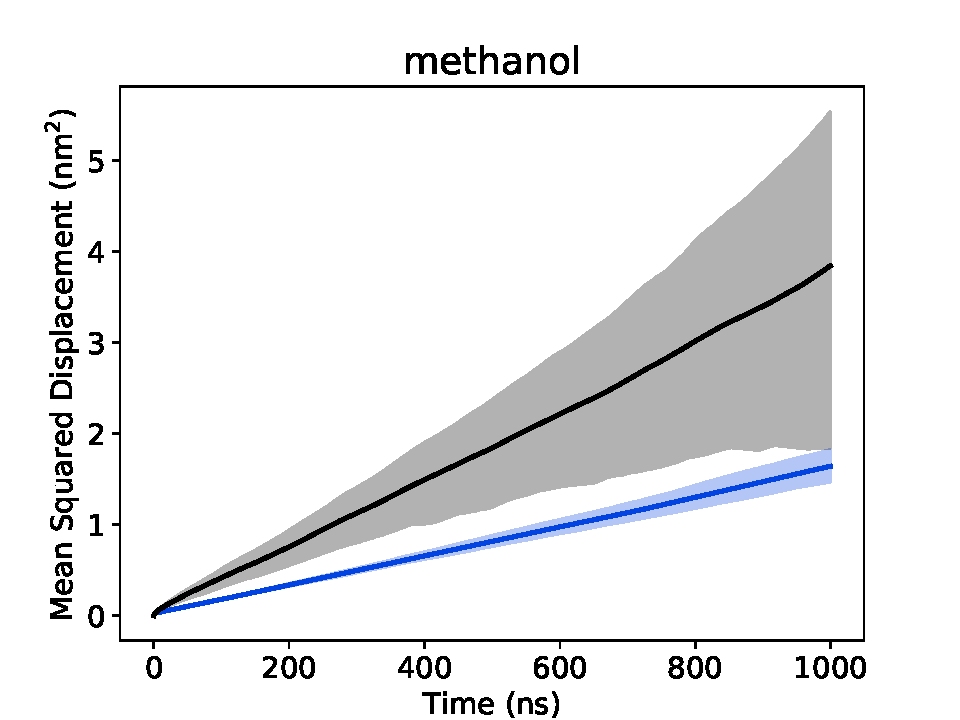
\includegraphics[width=\textwidth]{msd_MET.pdf}
  \caption{}\label{fig:msd_MET}
  \end{subfigure}
  \begin{subfigure}{0.45\textwidth}
  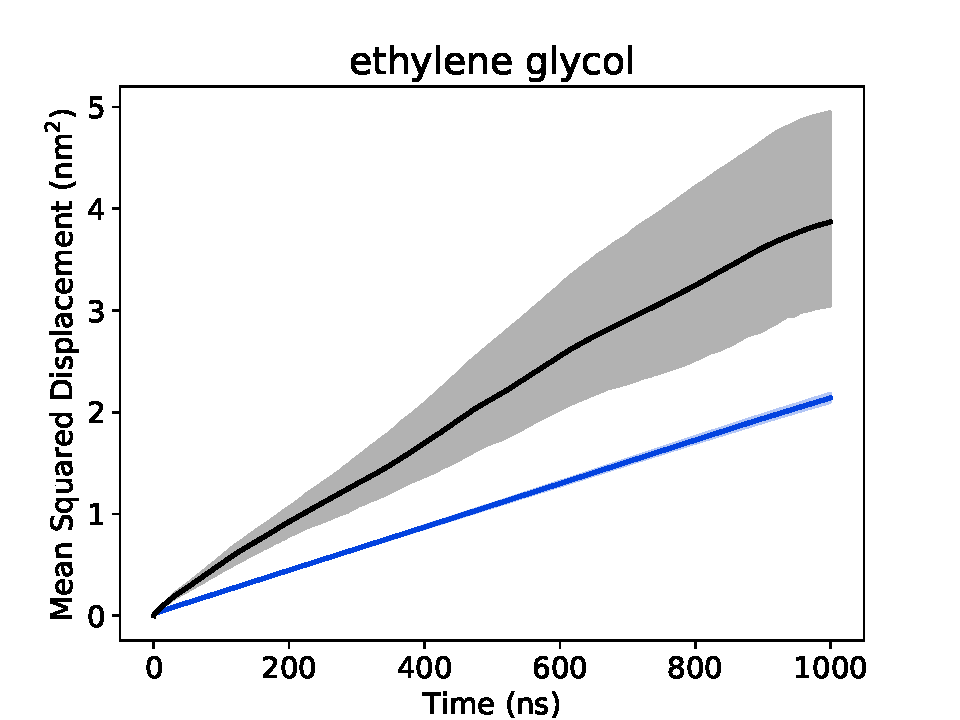
\includegraphics[width=\textwidth]{msd_GCL.pdf}
  \caption{}\label{fig:msd_GCL}
  \end{subfigure}
  \begin{subfigure}{0.45\textwidth}
  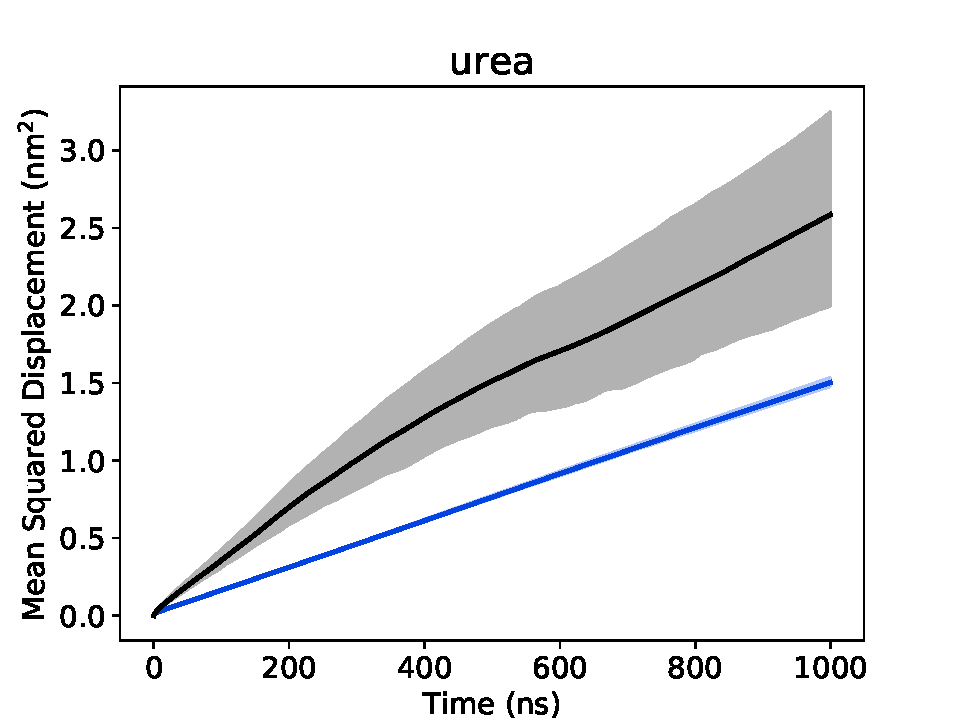
\includegraphics[width=\textwidth]{msd_URE.pdf}
  \caption{}\label{fig:msd_URE}
  \end{subfigure}
  \begin{subfigure}{0.45\textwidth}
  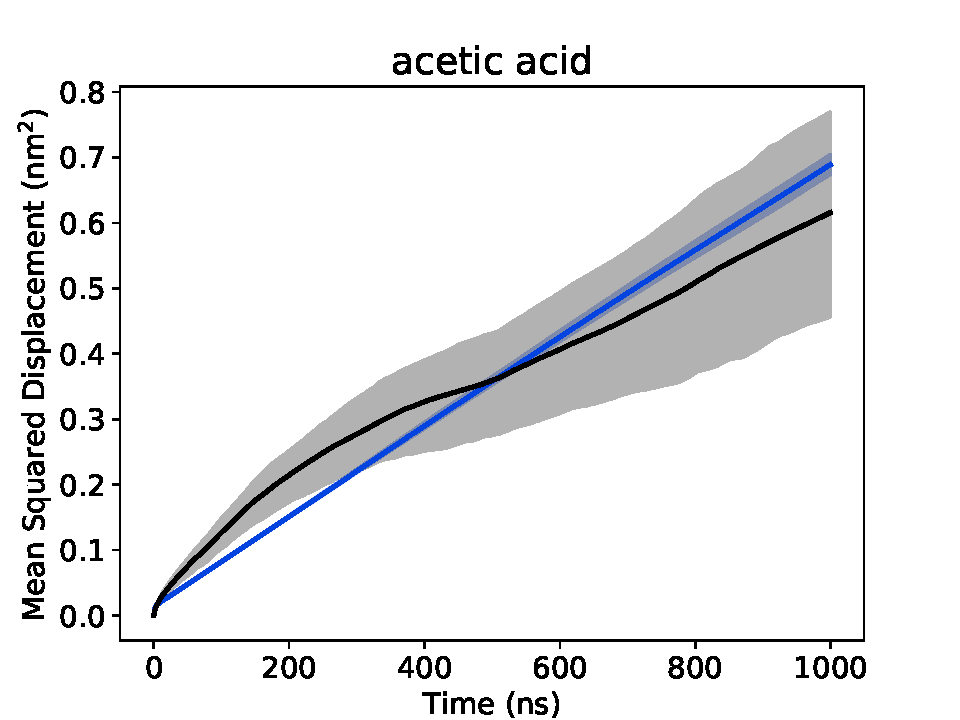
\includegraphics[width=\textwidth]{msd_ACH.pdf}
  \caption{}\label{fig:msd_ACH}
  \end{subfigure}
  \caption{The MSDs predicted based on 1000 realizations of our model (blue) tend to underpredict
  the MSDs based on the MD trajectories (black). Due to the variability in solute behavior across MD trajectories,
  as demonstrated in Figure~\ref{fig:trajectory_realizations_MET}, there are several 
  individual solute MSD curves that are significantly higher than the rest and drive up the
  mean of the MSD. If we remove those trajectories from the MSD calculation, we obtain 
  estimates much closer to the IHMM estimate.(I haven't done it yet, but could plot a third curve
  with outlier removed). Acetic acid, has no obvious outliers which is consistent with our model's
  prediction which lies within the 1$\sigma$ confidence interval of MD after a 1000 ns time lag.}\label{fig:msds}
  \end{figure}
  
  % BJC3: maybe need to talk about the curvature. Our model shouldn't have noticeable
  % curvature because it's only correlated with one step
  
  \section{Conclusion}
  
  We have shown that the IHMM can be used to automatically parameterize solute 
  time series with an unknown number of latent dynamical modes. Initially, we applied
  the algorithm to each trajectory independently. For each solute studied, this resulted
  in over 300 distinct states. By clustering the parameter sets we were able to reduce 
  the state space to 10\% of its original size by grouping states with similar VAR
  parameters.
  
  We coupled analysis of the clustered parameter sets with measurements of membrane 
  properties and solute-membrane interactions in order to gain a detailed understanding
  of the diverse sets behavior exhibited by solutes in these membranes. We showed how
  solute motion is influenced by hydrogen bonding, sodium ion association and local
  membrane density. These interactions have a direct impact on the size and
  correlation of sequential solute steps.
  
  % BJC6: I'll weaken this for the thesis, but this is what I hope to say in the 
  % final paper.
  Finally, we show how one can generate stochastic realizations of our model that
  can qualitatively and quantitatively reproduce the behavior of MD solute 
  trajectories. The realizations show the hopping and trapping behavior that is
  characteristic of polar solutes in this system. We can also use them to reproduce
  the solute MSDs measured from the MD trajectories. The low computational expense 
  of generating these stochastic trajectories allows one to project solute behavior
  on much longer timescales and thus predict experimentally-relevant macroscopic 
  transport properties like solute flux and selectivity.
  
  We showcase this modeling approach by example, but it is important to
  recognize the generality of this analysis, especially in the context of molecular
  simulations. Vector autogregressive models can describe a diverse set of behavior
  and so the IHMM may be suited to study many types motion, including those not 
  characterized by hopping and trapping. The IHMM is a powerful approach for 
  understanding particle motion as well as for generating cheap models
  which can give macroscopic insight.
  
  \section*{Supporting Information}

  Detailed explanations and expansions upon the results and procedures mentioned in
  the main text are described in the Supporting Information. This information is
  available free of charge via the Internet at http://pubs.acs.org.

  \section*{Acknowledgments}

  %MRS2: add GAANN and PRF here to cover bases.
  This work was supported in part by the ACS Petroleum Research Fund
  grant \#59814-ND7 and the Graduate Assistance in Areas of National Need (GAANN) 
  fellowship which is funded by the U.S. Department of Education. 
  Molecular simulations were performed using the Extreme Science and
  Engineering Discovery Environment (XSEDE), which is supported by National
  Science Foundation grant number ACI-1548562. Specifically, it used the Bridges
  system, which is supported by NSF award number ACI-1445606, at the Pittsburgh
  Supercomputing Center (PSC). This work also utilized the RMACC Summit supercomputer,
  which is supported by the National Science Foundation (awards ACI-1532235 and
  ACI-1532236), the University of Colorado Boulder, and Colorado State
  University. The Summit supercomputer is a joint effort of the University of
  Colorado Boulder and Colorado State University.

  \clearpage

  \bibliographystyle{ieeetr}
  \bibliography{hdphmm}

  %\newpage

  %\section*{TOC Graphic}

\end{document}

% LocalWords:  BJC micropollutants Desalination permeability nanofiltration LLC
% LocalWords:  Amphiphilic nanostructures Lyotropic amphiphilic lyotropic MSDDM
% LocalWords:  solutes selectivities solute nanoscopic timescales MSDs MSD HMMs
% LocalWords:  nonparameteric Parrinello Rahman barostat rescale transitioning
% LocalWords:  al's HMM Dirichlet HDP DP Wishart TODO SI al MATLAB teh gael pdf
% LocalWords:  nonparametric bayesian solute's reparameterized intracluster ca
% LocalWords:  delocalize Luzar Chandler histogrammed interpolator methanol's
% LocalWords:  nanostructure carboxylate VMD nonidealities hbonds outlier GAANN
% LocalWords:  autogregressive PRF ACS XSEDE ACI
